\chapter{Criptografia}


A palavra criptografia ~\cite{tanenbaum} vem das palavras gregas que significam "escrita secreta"~. A criptografia tem  uma longa e interessante história de milhares de anos. 
Os diversos  profissionais fazem distinção entre cifras e códigos. Uma cifra é uma transformação de caractere por caractere ou de bit por bit, sem levar em conta a estrutura lingüística da mensagem. Em contraste, um código substitui uma palavra por outra palavra ou símbolo. Os códigos não são mais utilizados, embora tenham uma história gloriosa. O código mais bem-sucedido já inventado foi usado pelas forças armadas dos Estados Unidos durante a Segunda Guerra Mundial no Pacífico. 
Eles simplesmente tinham índios Navajo que se comunicam uns com os outros usando palavras Navajo específicas para termos militares como, por exemplo, chay-dagahi-nail-tsaidi para indicar uma arma antitanque. A linguagem Navajo é altamente tonal, extremamente complexa, e não tem nenhuma forma escrita. 

\section{Introdução a Criptografia}

Quatro grupos de pessoas utilizaram e contribuíram para a arte da criptografia: 
\begin{itemize}
\item  os militares;
\item   os diplomatas; 
\item  as pessoas que gostam de guardar memórias;
\item  amantes;
\end{itemize}
Dentre eles, os militares tiveram o papel mais importante e definiram as bases para a tecnologia. Dentro das organizações militares, tradicionalmente as mensagens a serem criptografadas são entregues a auxiliares mal remunerados que se encarregam de criptografá-las e transmiti-las. O grande volume de mensagens impedia que esse trabalho fosse feito por alguns poucos especialistas. 
Até o advento dos computadores, uma das principais restrições impostas à criptografia era a 
habilidade do auxiliar de criptografia fazer as transformações necessárias, em geral com poucos equipamentos e no campo de batalha. Uma outra restrição era a dificuldade de alternar os métodos criptográficos rapidamente, pois isso exigia a repetição do treinamento de um grande número de pessoas. No entanto, o perigo de um auxiliar de criptografia ser capturado pelo inimigo tornou indispensável a possibilidade de se alterar o método criptográfico  se necessário.

\begin{figure}
\begin{center}
	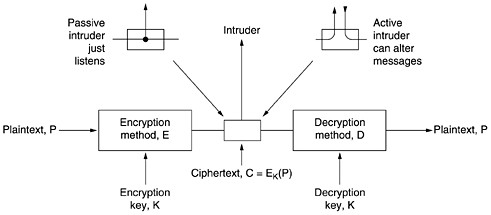
\includegraphics[width=0.7\textwidth]{criptografia1}
\end{center}
\caption{Criptografia~\cite{tanenbaum}}
\label{fig: criptografia}
\end{figure}


As mensagens a serem criptografadas, conhecidas como texto simples, são transformadas por uma 
função que é parametrizada ~\cite{tanenbaum} por uma chave. Em seguida, a saída do processo de criptografia, conhecida como texto cifrado, é transmitida, normalmente através de um mensageiro ou por rádio. Presumimos que o inimigo, ou intruso, ouça e copia cuidadosamente o texto cifrado completo. No entanto, ao contrário do destinatário pretendido, ele não conhece a chave para descriptografar o texto e, portanto, não pode fazê-lo com muita facilidade. Às vezes, o intruso pode  não só escutar o que se passa no canal de comunicação (intruso passivo), como também pode  gravar mensagens e reproduzi-las mais tarde, injetar suas próprias mensagens ou modificar mensagens legítimas antes que elas cheguem ao receptor (intruso ativo). A arte de solucionar mensagens cifradas é chamada criptoanálise. A arte de criar mensagens cifradas (criptografia) e solucioná-las (criptoanálise) é chamada coletivamente criptologia. 

Com freqüência, será útil e prático ter uma notação para estabelecer uma relação entre o texto 
simples, o texto cifrado e as chaves. Utilizaremos C = E K (P) para denotar que a criptografia do texto simples ~\cite{tanenbaum} P usando a chave K gera o texto cifrado C. Da mesma forma, P = D K (C) representa a descriptografia de C para se obter o texto simples outra vez. Então, temos: 
D K (E K (P)) = P 

Essa notação sugere que E e D são simplesmente funções matemáticas, o que é verdade. A única 
parte complicada é que ambas são funções de dois parâmetros, e escrevemos um desses 
parâmetros (a chave) como um caractere subscrito, em vez de representá-lo como um argumento, 
para distingui-lo da mensagem. 
Uma regra fundamental da criptografia é que se deve supor que o criptoanalista conhece os 
métodos genéricos de criptografia e descriptografia que são utilizados. Em outras palavras, o 
criptoanal ista sabe como funciona o método de criptografia. O esforço necessário para criar, testar e instalar um novo algoritmo toda vez que o antigo método (supostamente) é comprometido sempre dificultou a manutenção desse segredo. 
Imaginar que o algoritmo de criptografia é secreto quando ele não é resulta em mais prejuízo do que em benefícios.


É nesse ponto que entra a chave. A chave consiste em um string (relativamente) curto que 
seleciona uma das muitas formas possíveis de criptografia. Ao contrário do método genérico, que só pode ser modificado a cada período de alguns anos, a chave pode ser alterada sempre que 
necessário. Portanto, nosso modelo básico é um método genérico publicamente conhecido, 
parametrizado por uma chave secreta que pode ser alterada com facilidade. A idéia de que o 
cripto-analista conhece os algoritmos e que o segredo reside exclusivamente nas chaves é chamada princípio Kerckhoff, que recebeu esse nome em homenagem ao criptógrafo militar flamengo Auguste Kerckhoff ~\cite{tanenbaum} que e enunciou primeiro em 1883. Desse modo, temos: 
Princípio de Kerckhoff: Todos os algoritmos devem ser públicos; apenas as chaves são secretas. 


Devemos enfatizar o caráter não sigiloso do algoritmo. Tentar manter o algoritmo secreto, uma estratégia conhecida no ramo como segurança pela obscuridade, nunca funciona. Além disso, ao tornar o algoritmo público, o especialista em criptografia se livra de te de consultar inúmeros criptólogos ansiosos por decodificar o sistema para poderem publicar artigos demonstrando sua esperteza e inteligência. Caso muitos especialistas tenham tentado decodificar o algoritmo durante cinco anos após sua publicação e nenhum tenha obtido sucesso, isso provavelmente significa que o algoritmo é sólido. 

Na verdade, o sigilo está na chave, e seu tamanho é uma questão muito importante do projeto. 
Considere um bloqueio de combinação simples. Segundo o princípio geral, você insere dígitos em 
sequência. Todo mundo sabe disso, mas a chave é secreta. Uma chave com um tamanho de dois 
dígitos significa que existem 100 possibilidades, uma chave de três dígitos significa mil 
possibilidades e uma chave de seis dígitos significa um milhão de possibilidades. Quanto maior for a chave, mais alto será o fator de trabalho com que o cripto-analista terá de lidar. O fator de trabalho para decodificar o sistema através de uma exaustiva pesquisa no espaço da chave é exponencial em relação ao tamanho da chave. O sigilo é decorrente da presença de um algoritmo forte (mas público) e de uma chave longa. Para impedir que o seu irmãozinho leia suas mensagens de correio eletrônico, serão necessárias chaves de 64 bits. Para uso comercial de rotina, devem ser usados pelo menos 128 bits. Para manter o governo de outros países à distância, são necessárias chaves de pelo menos 256 bits, de preferência maiores.


Do ponto de vista do cripto-analista, o problema da criptoanálise apresenta três variações 
principais. Quando tem um de terminado volume de texto cifrado mas nenhum texto simples, o 
analista é confrontado com o problema de haver somente texto cifrado. Os criptogramas da seção 
de palavras cruzadas do jornal são um exemplo desse tipo de problema. Quando há uma 
correspondência entre o texto cifrado e o texto simples, o problema passa a ser chamado texto 
simples conhecido. Por fim, quando o cripto-analista tem a possibilidade de codificar trechos do texto simples escolhidos por ele mesmo, temos o problema do texto simples escolhido. Os 
criptogramas dos jornais poderiam ser decodificados de forma trivial se o cripto-analista tivesse a permissão de fazer perguntas tais como: Qual é a criptografia de ABCDEFGHIJKL? 
Com frequência, os novatos na área de criptografia pressupõem que, se uma cifra puder resistir a uma estratégia de texto cifrado, isso significa que ela é segura. Essa suposição é muito ingênua. 

Em muitos casos, o criptoanalista pode fazer uma estimativa com base em trechos do texto 
simples. Por exemplo, a primeira mensagem que muitos sistemas de tempo compartilhado emitem 
quando você os chama é "LOGIN:". Equipado com alguns pares de texto simples/texto cifrado, o 
trabalho do criptoanalista se torna muito mais fácil. Para obter segurança, o autor da criptografia deve ser conservador e se certificar de que o sistema seja inviolável, mesmo que seu oponente seja capaz de criptografar o texto simples escolhido. 
Historicamente, os métodos de criptografia têm sido divididos em duas categorias: as cifras de 
substituição e as cifras de transposição. Em seguida, trataremos de cada uma dessas técnicas 
como informações básicas para a criptografia moderna.



\section{Cifras de Substituição}

Em uma cifra de substituição ~\cite{tanenbaum}, cada letra ou grupo de letras é substituído por outra letra ou grupo de letras, de modo a criar um "disfarce". Uma das cifras mais antigas é a cifra de César, atribuída a Júlio César. Nesse método, a se torna D, b se torna E, c se torna F,... e z se torna C. Por exemplo, ataque passaria a ser WDTXH. Nos exemplos, o texto simples é apresentado em letras minúsculas e o texto cifrado em letras maiúsculas. 
Uma ligeira generalização da cifra de César permite que o alfabeto do texto cifrado seja deslocado k letras, em vez de 3. Nesse caso, k passa a ser uma chave para o método genérico dos alfabetos deslocados em forma circular. A cifra de César pode ter enganado os cartagineses, mas nunca mais enganou ninguém. 
O próximo aprimoramento é fazer com que cada um dos símbolos do texto simples, digamos 26 
letras, seja mapeado para alguma outra letra. Por exemplo, 
texto simples: a b c d e f g h i j k l m n o p q r s t u v w x y z 
texto cifrado: Q W E R T Y U I O P A S D F G H J K L Z X C V B N M

Esse sistema geral é chamado substituição monoalfabética, sendo a chave o string de 26 letras 
correspondente ao alfabeto completo. Para a chave anterior, o texto simples ataque seria 
transformado no texto cifrado QZQJXT. 
À primeira vista, talvez esse sistema pareça seguro, pois apesar de conhecer o sistema genérico (substituição de letra por letra), o criptoanalista não sabe qual das 26 chaves possíveis está em uso. Ao contrário do que acontece com a cifra de César, experimentar todas elas não é uma estratégia muito interessante. Mesmo a 1 ns por solução, um computador levaria 10 elevado a 10 anos para experimentar todas as chaves. 

Todavia, com um volume de texto cifrado surpreendentemente pequeno, a descoberta com facilidade. A estratégia básica se beneficia das propriedades idiomas. Por exemplo, em inglês e é a letra mais comum, seguida de t, o, combinações de duas letras, ou digramas, mais comuns são th, in, er, re e an. As três letras, ou trigramas, mais comuns são the, ing, and e ion. cifra pode ser estatísticas dos a, n, i etc. As combinações de um criptoanalista que esteja tentando decodificar uma cifra monoalfabética começaria contando as freqüências relativas de todas as letras do texto cifrado. Depois disso, através de tentativas, ele atribuiria e à letra mais comum e t à próxima letra mais comum. Em seguida, verificaria os trigramas para encontrar um no formato tXe, o que poderia sugerir que X é h. Da mesma forma, se o padrão thYt ocorrer com freqüência, provavelmente isso significará que Y representa a. Com essas informações, o criptoanalista poderá procurar por um trigrama com o formato aZW que ocorra com freqüência (muito provavelmente and). Fazendo estimativas em relação a digramas, trigramas e letras mais comuns, e conhecendo os prováveis padrões de vogais e consoantes, o criptoanalista criaria um texto simples através de tentativas, letra por letra. 
Outra estratégia é adivinhar uma palavra ou frase provável. Por exemplo, considere o seguinte 
texto cifrado de uma empresa de contabilidade (montado em grupos de cinco caracteres): 
	

CTBMN BYCTC BTJDS QXBNS GSTJC BTSWX CTQTZ CQVUJ 
QJSGS TJQZZ MNQJS VLNSX VSZJU JDSTS JQUUS JUBXJ 
DSKSU JSNTK BGAQJ ZBGYQ TLCTZ BNYBN QJSW 


Nos Estados Unidos, uma palavra muito provável em uma mensagem de uma empresa de contabilidade é financial. Utilizando nosso conhecimento de que inancial tem um caractere repetido (i), com quatro outras letras entre suas ocorrências, estamos procurando letras repetidas no texto cifrado com esse espaço entre elas. Encontramos 12 casos como esse nas posições 6, 15, 27, 31, 42, 48, 56, 66, 70, 71, 76 e 82. No entanto, apenas dois deles, 31 e 42, têm a letra seguinte (que corresponde a n no texto simples) repetida na localização adequada. Dessas duas, apenas 31 também tem a letra a corretamente posicionada; portanto, sabemos que financial começa na posição 30. Desse ponto em diante, fica fácil deduzir a chave utilizando a estatística de freqüência para o texto em inglês.


\section {Cifras de Transposição}

As cifras de substituição ~\cite{tanenbaum} preservam a ordem dos símbolos no texto simples, mas disfarçam essessímbolos. Por outro lado, as cifras de transposição reordenam as letras, mas não as disfarçam.  A cifra se baseia em uma chave que é uma palavra ou frase que não contém letras repetidas. Nesse exemplo, MEGABUCK é a chave. O objetivo da chave é numerar as colunas de modo que a coluna 1 fique abaixo da letra da chave mais próxima do início do alfabeto e assim por diante. O texto simples é escrito horizontalmente, em linhas. O texto cifrado é lido em colunas, a partir da coluna cuja letra da chave seja a mais baixa.


\begin{figure}
	\begin{center}
		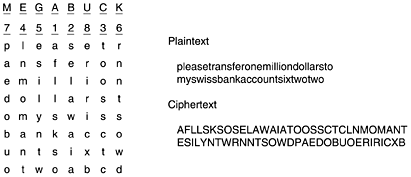
\includegraphics[width=0.7\textwidth]{criptografia2}
	\end{center}
	\caption{Transposição ~\cite{tanenbaum}}
	\label{fig:criptografia2}
\end{figure}

Para romper uma cifra de transposição, o criptoanalista deve primeiro estar ciente de que está
lidando com uma cifra de transposição. Examinando a freqüência de E, T, A, O, I, N etc., fica fácil constatar se essas letras se encaixam no padrão normal para texto simples. Se houver
correspondência, isso significa que a cifra é evidentemente uma cifra de transposição, pois nesse tipo de cifra cada letra é representada por ela mesma, mantendo intacta a distribuição de freqüências.
A próxima etapa é fazer uma estimativa do número de colunas. Em muitos casos, uma palavra ou
frase provável pode ser deduzida a partir do contexto da mensagem. Por exemplo, suponha que o
nosso criptoanalista tenha suspeitado de que a frase em texto simples milliondollars ocorre em
algum lugar na mensagem. Observe que os digramas MO, IL, LL, LA, IR e OS ocorrem no texto
cifrado como um resultado do desdobramento dessa frase. No texto cifrado, a letra O vem depois
da letra M (ou seja, elas são verticalmente adjacentes na coluna 4), pois estão separadas na
provável frase por uma distância igual ao tamanho da chave. Se tivesse sido usada uma chave de
tamanho sete, teriam surgido os digramas MD, IO, LL, LL, IA, OR e NS. Na verdade, para cada
tamanho de chave, é produzido um conjunto de digramas diferente no texto cifrado. Ao tentar
encontrar diferentes possibilidades, muitas vezes o criptoanalista é capaz de determinar com
facilidade o tamanho da chave.
A última etapa é ordenar as colunas. Quando o número de colunas k é pequeno, cada um dos k(k -
1) pares de colunas pode ser examinado para que seja constatado se suas freqüências de digramas correspondem às do texto simples em inglês. O par que tiver a melhor correspondência será considerado na posição correta. Em seguida, cada uma das colunas restantes é experimentada como sucessora desse par. A coluna cujas freqüências de digramas e trigramas proporcione a melhor correspondência será experimentalmente considerada correta. O processo inteiro continua até ser encontrada uma ordenação potencial. O mais provável é que o texto simples seja reconhecido nesse ponto (por exemplo, se ocorrer milloin, ficará claro qual é o erro).

Algumas cifras de transposição aceitam um bloco de tamanho fixo como entrada e produzem um
bloco de tamanho fixo como saída. Essas cifras podem ser completamente descritas fornecendo-se
um a lista que informe a ordem na qual os caracteres devem sair. Por exemplo, a cifra da Figura 5.2 pode ser vista como uma cifra de blocos de 64 caracteres. Sua saída é 4, 12, 20, 28, 36, 44, 52, 60,5, 13,..., 62. Em outras palavras, o quarto caractere de entrada, a, é o primeiro a sair, seguido pelo décimo segundo, f, e assim por diante.


\section{Chave Única - One-Time Pad}

Um oficial do Exército dos Estados Unidos, Joseph Mauborgne, propôs uma melhora na cifra de Vernam ~\cite{stallings}, que gera o máximo em segurança. Esse oficial sugeriu o uso de uma chave aleatória que fosse tão grande quanto a mensagem, de modo que a chave não precisasse ser repetida e essa chave permite criptografar e decriptografar a mensagem, assim esse esquema é inquebrável. Ele produz uma saída aleatória que não possui nenhum relacionamento estatístico com o texto claro.

\begin{figure}
	\begin{center}
		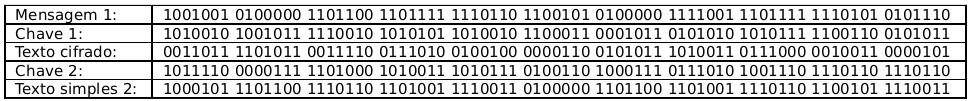
\includegraphics[width=0.7\textwidth]{criptografia3}
	\end{center}
	\caption{Chave Única ~\cite{tanenbaum}}
	\label{fig: criptografia3}
\end{figure}

Na verdade, é fácil criar uma cifra inviolável ~\cite{tanenbaum} a técnica é conhecida há décadas. Primeiro, escolha como chave um string de bits aleatórios. Em seguida, converta o texto simples em um string de bits, utilizando por exemplo sua representação ASCII. Por fim, calcule o OR exclusivo (X OR) desses dois strings. O texto cifrado resultante não pode ser violado porque, em uma amostra suficientemente grande de texto cifrado, cada letra ocorrerá com a mesma freqüência, bem como digrama, cada trigrama e assim por diante. Esse método, conhecido como chave única, é imune a todos os ataques presentes e futuros, quanta capacidade computacional tenha o intruso. A razão deriva da teoria da informação: simplesmente não existe nenhuma informação na mensagem, todos os textos simples possíveis com o tamanho dado são igualmente prováveis. Um exemplo de como as chaves únicas são usadas, é dado na \ref{fig: criptografia3}. 




Primeiro, a mensagem 1, "I love you", é convertida em ASCII de 7 bits. Em seguida, uma chave única chamada chave 1, é escolhida e sujeita à operação XOR com a mensagem para se obter o texto cifrado.Um criptoanalista poderia experimentar todas as chaves únicas possíveis para ver que texto resultou para cada uma. Por exemplo, a chave única listada como chave 2 na figura poderia ser experimentada, resultando no texto simples 2, "Elvis lives", que pode ser ou não plausível. De fato, para cada texto simples ASCII de 11 caracteres, existe uma chave única que o gera. É isso que quero dizer quando mencionamos que não existe nenhuma informação no texto cifrado: é possível obter qualquer mensagem com o tamanho correto a partir dele.
 
 
 \section{Criptografia Quântica}
 
 É interessante observar que talvez haja uma solução para o problema de como transmitir a chave única pela rede, e ela vem de uma fonte muito improvável: a mecânica quântica. Essa área ainda é experimental, mas os testes iniciais são promissores. Se eles puderem ser aperfeiçoados e se tornarem eficientes, quase toda a criptografia será realizada eventualmente com a utilização de chaves únicas ~\cite{tanenbaum}, pois elas talvez sejam seguras. A seguir, explicaremos em linhas gerais como funciona esse método, denominado criptografia quântica. Em particular, descreveremos um protocolo chamado BB84 para indicar seus autores e o ano da publicação (Bennet e Brassard, 1984).

Uma usuária chamada Alice quer estabelecer uma chave única com um segundo usuário, Bob. Alice
e Bob são chamados protagonistas, os personagens principais de nossa história. Por exemplo, Bob é um banqueiro com quem Alice gostaria de realizar negócios. Os nomes "Alice" e "Bob " foram usados como protagonistas em praticamente todos os ensaios e livros sobre criptografia na última década. Os criptógrafos amam a tradição. Se fôssemos usar "Andy" e "Barbara" como
protagonistas, ninguém acreditaria em nada do que fosse explicado aqui. Então, que seja!
Se Alice e Bob pudessem estabelecer uma chave única, eles teriam a possibilidade de empregá-la
para se comunicarem com segurança. A pergunta é: como eles podem estabelecê-la sem
anteriormente troca DVDs? Podemos supor que Alice e Bob estão em extremidades opostas de um
cabo de fibra óptica pelo qual podem enviar e receber pulsos de luz. Porém, uma intrépida intrusa chamada Trudy pode cortar a fibra e criar um grampo ativo. Trudy pode ler todos os bits em ambos os sentidos.
Ela também pode enviar falsas mensagens nos dois sentidos. A situação pode parecer desesperada para Alice e Bob, mas a criptografia quântica pode trazer uma nova luz sobre o assunto.
A criptografia quântica ~\cite{tanenbaum} se baseia no fato de que a luz se propaga em pequenos pacotes chamadosfótons, que apresentam algumas propriedades peculiares. Além disso, a luz pode ser polarizada ao passar por um filtro de polarização, um fato bem conhecido para os usuários de óculos de sol e fotógrafos. Se um feixe de luz (isto é, um fluxo de fótons) passar por um filtro de polarização, todos os fótons que emergirem dele serão polarizados na direção do eixo do filtro (por exemplo, vertical).Se o feixe passar agora por um segundo filtro de polarização, a intensidade da luz que emergirá do segundo filtro será proporcional ao quadrado do cosseno do ângulo entre os eixos. Se os dois eixos forem perpendiculares, nenhum fóton passará pelo filtro. A orientação absoluta dos dois filtros não importa; só interessa o ângulo entre seus eixos.
Para gerar uma chave única, Alice precisa de dois conjuntos de filtros de polarização. O primeiro conjunto consiste em um filtro vertical e um filtro horizontal. Essa escolha é chamada base retilínea. Uma base é apenas um sistema de coordenadas. O segundo conjunto de filtros é idêntico, exceto por estar deslocado 45 graus, de forma que um filtro abrange desde o canto inferior esquerdo até o canto superior direito, e o outro filtro abrange desde o canto superior esquerdo até o canto inferior direito. Essa escolha é chamada base diagonal. Desse modo, Alice tem duas bases, que ela pode inserir rapidamente em seu feixe à vontade. Na realidade, Alice não tem quatro filtros separados, mas um cristal, cuja polarização pode ser trocada eletricamente para qualquer das quatro direções permitidas, em alta velocidade. Bob tem o mesmo equipamento de Alice. O fato de Alice e Bob terem cada um duas bases disponíveis é essencial para a criptografia quântica ~\cite{tanenbaum}.
Para cada base, Alice atribui agora uma direção como 0 e a outra como 1. No exemplo apresentado a seguir, supomos que ela escolhe a direção vertical como 0 e a horizontal como 1. Independente mente, ela também escolhe do canto inferior esquerdo até o canto superior direito como 0, e do canto superior esquerdo até o canto inferior direito como 1. Alice envia essas escolhas a Bob como texto simples.

Agora, Alice escolhe uma chave única, por exemplo com base em um gerador de números
aleatórios (um assunto por si só bastante complexo). Ela o transfere bit por bit para Bob,
escolhendo uma de suas bases ao acaso para cada bit. Para enviar um bit, sua pistola de fótons
emite um fóton polarizado de maneira apropriada, conforme a base que ela está usando para esse
bit. Por exemplo, ela poderia escolher as bases diagonal, retilínea, retilínea, diagonal, retilínea etc. Para enviar sua chave única igual a 1001110010100110 com essas bases, ela enviaria os fótons mostrados na \ref{fig: criptografia3}. Dada a chave única e a seqüência de bases, a polarização a ser usada para cada bit é determinada de forma exclusiva. Bits enviados um fóton de cada vez são chamados qubits.

\begin{figure}
	\begin{center}
		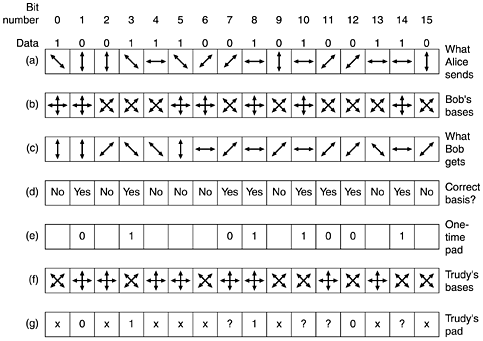
\includegraphics[width=0.7\textwidth]{criptografia4}
	\end{center}
	\caption{Criptografia Quântica ~\cite{tanenbaum}}
	\label{fig:criptografia4}
\end{figure}

Bob não sabe que base usar, e assim escolhe uma base ao acaso para cada fóton que chega e
simplesmente o utiliza, como mostra a \ref{fig:criptografia4}. Se escolher a base correta, ele receberá o bit correto. Se escolher a base incorreta, ele receberá um bit aleatório porque, se um fóton acessar um filtro polarizado a 45 graus em relação à sua própria polarização, ele saltará ao acaso para a polarização do filtro ou para uma polarização perpendicular à do filtro, com igual probabilidade.
Essa propriedade dos fótons é fundamental para a mecânica quântica. Desse modo, alguns bits estão corretos e alguns são aleatórios, mas Bob não consegue distingui-los. Os resultados de Bob  estão representados na \ref{fig:criptografia4}.
De que maneira Bob pode descobrir quais são as bases corretas e quais são as erradas entre as
que recebeu? Ele simplesmente diz a Alice que base usou para cada bit em texto simples, e ela diz quais são as bases corretas e quais são as erradas em texto simples, como mostra a \ref{fig:criptografia4}. A partir dessas informações, ambos podem construir um stri ng de bits com os palpites
corretos, como mostra a \ref{fig:criptografia4}. Em média, esse string de bits terá metade do comprimento do string de bits original mas, como ambas as partes o conhecem, elas poderão usá-lo como uma chave única. Tudo que Alice tem a fazer é transmitir um string de bits um pouco maior que o dobro do tamanho desejado, para que ela e Bob tenham uma chave única com o comprimento apropriado.
Porém, espere um minuto. Esquecemos de Trudy. Vamos supor que ela esteja curiosa para saber o
que Alice tem a dizer e corte o cabo de fibra, inserindo seu próprio detector e transmissor.
Infelizmente para Trudy, ela também não sabe que base usar para cada fóton. O melhor que ela
pode fazer é escolher uma base ao acaso para cada um dos fótons, como fez Bob. Um exemplo de
suas escolhas é mostrado na \ref{fig:criptografia4}. Quando mais tarde Bob informar (em texto simples) que
bases usou e Alice disser a ele (em texto simples) quais delas estão corretas, Trudy saberá quando acertou e quando errou. Na Figura 5.4, ela acertou nos bits 0, 1, 2, 3, 4, 6, 8, 12 e 13. No entanto, ela sabe pela resposta de Alice na Figura 5.4 que só os bits 1, 3, 7, 8, 10, 11, 12 e 14 fazem parte da chave única. Em quatro desses bits (1, 3, 8 e 12), ela acertou seu palpite e captou o bit correto. Nos outros quatro (7, 10, 11 e 14), ela e rrou e não sabe qual bit foi transmitido. Desse modo, Bob sabe que a chave única ~\cite{tanenbaum} começa com 01011001, a parir da Figura 5.4(e), mas tudo que Trudy tem é 01?1??0?, a partir da \ref{fig:criptografia4}.

É claro que Alice e Bob estão cientes de que Trudy talvez tenha captado parte de sua chave única, e assim gostariam de reduzir as informações que Trudy tem. Eles podem fazer isso executando uma transformação na chave. Por exemplo, poderiam dividir a chave única em blocos de 1024 bits e elevar ao quadrado cada uma para formar um número de 2048 bits, usando a concatenação desses números de 2048 bits como a chave úni ca. Com seu conhecimento parcial do string de bits transmitido, Trudy não tem como gerar seu quadrado e, portanto, não tem nada. A transformação da chave única original em uma chave diferente que reduz o conhecimento de Trudy é chamada amplificação da privacidade. Na prática, são usadas transformações complexas em que todo bit de entrada depende de cada bit de saída em lugar da elevação ao quadrado.
Pobre Trudy. Ela não apenas não tem nenhuma idéia de qual é a chave única, mas sua presença
não é mais secreta. Afinal, ela tem de retransmitir cada bit recebido para Bob, a fim de levá-lo a pensar que está se comunicando com Alice. Porém, o melhor que ela pode fazer é transmitir o qubitque recebeu, usando a mesma polarização que empregou para recebê-lo, e durante cerca de
metade do tempo ela estará errada, provocando muitos erros na chave única de Bob.

Quando finalmente começar a transmitir dados ~\cite{tanenbaum}, Alice os codificará usando um pesado código de
correção antecipada de erros. Do ponto de vista de Bob, um erro de 1 bit na chave única é o
mesmo que um erro de transmissão de 1 bit. De qualquer modo, ele receberá o bit errado. Se
houver correção antecipada de erros suficiente, ele poderá recuperar a mensagem original apesar de todos os erros, mas poderá contar com facilidade quantos erros foram corrigidos. Se esse número for muito maior que a taxa de erros esperada do equipamento, ele saberá que Trudy
grampeou a linha e poderá agir de acordo (por exemplo, informando a Alice que ela deve mudar
para um canal de rádio, chamar a polícia etc.). Se Trudy tivesse um meio de clonar um fóton, de forma que ela tivesse um fóton para inspecionar e um fóton idêntico para enviar a Bob, ela poderia evitar a detecção mas, no momento, não se conhece nenhum mo do perfeito de clonar um fóton.

No entanto, mesmo que Trudy pudesse clonar fótons, o valor da criptografia quântica para
estabelecer chaves únicas não seria reduzido. Embora a criptografia quântica opere sobre distâncias de até 60 km de fibra, o equipamento é complexo e dispendioso.

\section {Princípios Fundamentais de Criptografia}

Existem diversos sistemas criptográficos entretando é importante entendermos dois princípios básicos que norteia grande parte deste assunto. São eles:

\subsection {Redundâcia}

O primeiro princípio é que todas as mensagens criptografadas devem conter alguma redundância ~\cite{tanenbaum}, ou seja, informações que não são necessárias para a compreensão da mensagem. Talvez um exemplo esclareça por que isso é necessário. Considere uma empresa de encomendas postais, a The Couch Potato (TCP), com 60.000 produtos. Pensando que estavam sendo muito eficientes, os
programadores da TCP decidiram que as mensagens de encomendas deveriam consistir no nome
do cliente com 16 bytes, seguido por um campo de dados de 3 bytes (um para a quantidade e 2
para o número do produto). Os 3 últimos bytes devem ser criptografados por meio de uma chave
muito longa conhecida apenas pelo cliente e pela TCP.

Em princípio, essa estratégia pode parecer segura, e até certo ponto isso acontece, porque os
intrusos passivos não podem descriptografar as mensagens. Infelizmente, há uma falha fatal que a
torna inútil. Suponha que uma funcionária recém-demitida queira punir a TCP por despedi-la. Antes
de sair da empresa, ela leva consigo parte da lista de clientes e passa a noite acordada criando um
programa para gerar encomendas fictícias utilizando nomes de clientes verdadeiros. Como não tem
a lista das chaves, ela simplesmente inclui números aleatórios nos três últimos bytes e envia
centenas de encomendas para a TCP.

Quando as mensagens chegam, o computador da TCP utiliza o nome do cliente para localizar a
chave e descriptografar a mensagem. Infelizmente para a TCP, quase todas as mensagens de 3
bytes são válidas; portanto, o computador começa a imprimir as instruções de entrega. Apesar de
parecer estranho um cliente encomendar 837 conjuntos de balanços para crianças, ou 540 caixas
de areia, para o computador, o cliente pode estar planejando abrir uma cadeia de parques de
diversões franqueados. Portanto, um intruso ativo (a ex-funcionária) pode causar muitos
problemas, mesmo que não seja capaz de entender as mensagens que seu computador está
gerando.

Esse problema pode ser resolvido através da inclusão de informações redundantes em todas as
mensagens. Por exemplo, se as mensagens de pedidos forem ampliadas para 12 bytes, os 9
primeiros deverão ser iguais a zero; assim, essa estratégia de ataque deixa de ser interessante,
porque a ex-funcionária não é mais capaz de gerar um longo fluxo de mensagens válidas. A moral
da história é que todas as mensagens devem conter informações redundantes suficientes para que
os intrusos ativos sejam impedidos de transmitir dados inválidos que possam ser interpretados
como uma mensagem válida.

No entanto, a inclusão de informações redundantes também facilita a ruptura de mensagens por
parte dos criptoanalistas. Suponha que a empresa de encomenda postal seja muito competitiva e
esteja na posição de principal concorrente da The Couch Potato. A Sofa Tuber adoraria saber
quantas caixas de areia a TCP está vendendo. Portanto, a empresa resolve grampear a linha
telefônica da TCP. No esquema original com mensagens de 3 bytes, a criptoanálise era
praticamente impossível porque, após descobrir uma chave, o criptoanalista não era capaz de dizer
se a mensagem estava correta. Afinal de contas, quase todas as mensagens são tecnicamente
válidas. Com o novo esquema de 12 bytes, fica mais fácil para o criptoanalista distinguir uma
mensagem válida de uma inválida. Desse modo, temos:

Princípio criptográfico 1 ~\cite{tanenbaum}: as mensagens devem conter alguma redundância
Em outras palavras, ao decifrar uma mensagem, o destinatário deve ser capaz de saber se ela é
válida, simplesmente inspecionando-a e talvez executando uma computação simples. Essa
redundância é necessária para impedir que intrusos ativos enviem lixo e enganem o receptor,
fazendo-o descriptografar o lixo e agir sobre o "texto simples". No entanto, essa mesma
redundância permite que os intrusos passivos entrem no sistema com maior facilidade; portanto,
há uma zona de tensão nessa situação. Além disso, a redundância nunca deverá ser criada sob a
forma de n zeros no início ou no fim de uma mensagem, pois a submissão dessas mensagens a
determinados algoritmos criptográficos proporciona resultados mais previsíveis, facilitando o trab
alho do criptoanalista. Um polinômio de CRC é muito melhor que uma seqüência de valores 0, pois
o receptor pode verificá-lo facilmente, mas ele irá gerar mais trabalho para o criptoanalista. Seria
muito melhor usar um hash criptográfico, um conceito que exploraremos mais adiante.

Voltando à criptografia quântica por um momento, também podemos ver como a redundância
desempenha um papel importante. Devido à interceptação dos fótons por Trudy, alguns bits na
chave única de Bob estarão errados. Bob precisa de alguma redundância nas mensagens de
entrada para descobrir os erros presentes. Uma forma muito rudimentar de redundância é repetir a mensagem duas vezes. Se as duas cópias não forem idênticas, Bob saberá que a fibra está muito
ruidosa, ou que alguém está interferindo na transmissão. É claro que enviar tudo duas vezes é um
exagero; um código de Hamming ou de Reed-Solomon é um modo mais eficiente de realizar a
detecção e correção de erros. Porém, deve ficar claro que uma certa redundância é necessária para
distinguir uma mensagem válida de uma mensagem inválida, em especial diante de um intruso
ativo.

\subsection {Atualidade}

O segundo princípio criptográfico ~\cite{tanenbaum} é tomar algumas medidas para assegurar que cada mensagem recebida possa ser confirmada como uma mensagem atual, isto é, enviada muito recentemente.
Essa medida é necessária para impedir que intrusos ativos reutilizem mensagens antigas. Se tais
medidas não fossem tomadas, nossa ex-funcionária poderia interceptar a linha telefônica da TCP e
ficar simplesmente repetindo mensagens válidas já enviadas. Em outras palavras, essa idéia nos
diz que:
Princípio criptográfico 2: algum método é necessário para anular ataques de repetição
Uma medida desse tipo seria incluir em cada mensagem um timbre de hora válido apenas por,
digamos, 10 segundos. Em seguida, o receptor poderia manter as mensagens durante 10
segundos, a fim de comparar as mensagens recém-chegadas com as anteriores e filtrar duplicatas.
As mensagens transmitidas há mais de 10 segundos poderiam ser descartadas, pois as repetições
enviadas mais de 10 segundos depois da mensagem original serão rejeitadas por serem muito
antigas. Outras medidas além dos timbres de hora serão discutidas mais adiante.


\section {Algoritmos de Chave Simétrica}

Embora a criptografia moderna utilize as mesmas idéias básicas da criptografia tradicional
(transposição e substituição), sua ênfase é diferente. Tradicionalmente, as pessoas que criam a
criptografia têm utilizado algoritmos simples. Hoje em dia, acontece o invers o: o objetivo é tornar o algoritmo de criptografia tão complexo e emaranhado que, mesmo que o criptoanalista adquira
enormes volumes de texto cifrado de su a própria escolha, sem a chave ele não seja capaz de
captar qualquer sentido em tudo que conseguir.

A primeira classe de algoritmos de criptografia que estudaremos neste capítulo é a dos algoritmos
de chave simétrica, porque utilizam a mesma chave para codificação e decodificação. A Figura
8.2 ilustra o uso de um algoritmo de chave simétrica. Em particular, vamos nos concentrar nas
cifras de bloco, que obtêm um bloco de n bits de texto simples como entrada e o transformam
usando a chave em um bloco de n bits de texto cifrado.

Os algoritmos criptográficos podem ser implementados em hardware (para se obter velocidade) ou
em software (para se obter flexibilidade). Embora a maior parte de nosso tratamento esteja relaci
onado aos algoritmos e protocolos, que são independentes da implementação real, algumas
palavras sobre a construção de hardware criptográfico podem ser interessantes. As transposições e
substituições podem ser implementadas com circuitos elétricos simples. A Figura 4.5(a) mostra um
dispositivo, conhecido como caixa P (onde P significa permutação), usado para efetuar uma
transposição em uma entrada de 8 bits. Se os 8 bits forem designados de cima para baixo como
01234567, a saída dessa caixa P específica será 36071245. Com uma fiação interna adequada,
pode-se criar uma caixa P para executar qualquer transposição praticamente na velocidade da luz,
pois nenhuma computação é envolvida, apenas a propagação e sinais. Esse projeto segue o
princípio de Kerckhoff: o atacante sabe que o método geral é permutar os bits. O que ele não sabe
é qual bit fica em cada posição, e isso é a chave.


\begin{figure}
	\begin{center}
		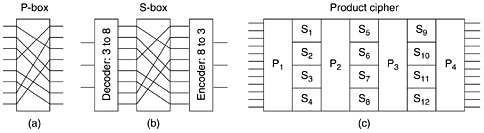
\includegraphics[width=0.7\textwidth]{criptografia6}
	\end{center}
	\caption{Criptografia Chave Simétrica \cite{tanenbaum}}
	\label{fig:criptografia6}
\end{figure}


\ref{fig:criptografia6}: Elementos básicos de cifras de produtos. (a) Caixa P. (b) Caixa S. (c) ProdutoAs substituições são realizadas por caixas S, como mostra a \ref{fig:criptografia6}). Nesse exemplo, é
introduzido um texto simples de 3 bits, e a saída é um texto cifrado de 3 bits. A entrada de 3 bits
seleciona uma das oito linhas de saída do primeiro estágio e a define como 1; todas as outras são
iguais a 0. O segundo estágio é uma caixa P. O terceiro estágio codifica a linha selecionada
novamente em binário. Com a fiação mostrada, se os oito números octais 01234567 fossem
introduzidos um após o outro, a seqüên cia de saída seria 24506713. Em outras palavras, 0 foi
substituído por 2, 1 foi substituído por 4 etc. Mais uma vez, com a fiação apropriada da caixa P
dentro da caixa S, qualquer substituição pode ser realizada. Além disso, tal dispositivo pode ser
construído em hardware e pode alcançar grande velocidade, pois os codificadores e os
decodificadores têm apenas um ou dois retardos de porta (subnanossegundo) e o tempo de
propagação pela caixa P pode ser menor que 1 picossegundo.

A capacidade real desses elementos básicos se torna aparente quando dispomos uma série inteira
de caixas em cascata para formar uma cifra de produto, como mostra a 
\ref{fig:criptografia6}. Nesse
exemplo, 12 linhas de entrada são transpostas (isto é, permutadas) pelo primeiro estágio (P1).
Teoricamente, seria possível fazer com que o segundo estágio fosse uma caixa S que mapeasse um
número de 12 bits em outro número de 12 bits. No entanto, tal dispositivo necessitaria de 2 12 =
4096 fios cruzados em seu estágio intermediário. Em vez disso, a entrada é dividida em quatro
grupos de 3 bits, sendo que cada um deles é substituído de forma independente dos outros. Apesar
de ser menos genérico, esse método ainda é mais eficiente. Através da inclusão de um número de
estágios suficientemente grande na cifra de produto, a saída pode ser transformada em uma
função excessivamente complicada da entrada.

As cifras de produto que operam sobre entradas de k bits para produzir saídas de k bits são muito
comuns. Em geral, o valor de k varia de 64 a 256. Uma implementação de hardware normalmente
tem pelo menos 18 estágios físicos, em vez de apenas sete, como na Figura 4.5(c). Uma
implementação de software é programada como um loop com pelo me nos 8 iterações, cada uma
executando substituições semelhantes às de caixas S em sub-blocos do bloco de dados de 64 bits a
256 bits, seguidas por uma permutação que mistura as saídas das caixas S. Com freqüência, existe
uma permutação especial no início e também uma no fim. Na literatura, as repetições são
chamadas rodadas.

\section {DES - \emph{Data Encryption Standard}}


Em janeiro de 1977, o governo dos Estados Unidos adotou uma cifra de produto desenvolvida pela
IBM como seu padrão oficial para informações não confidenciais. A cifra, DES ~\cite{greg} (Data Encryption Standard — padrão de criptografia de dados), foi amplamente adotada pelo setor de informática para uso em produtos de segurança. Em sua forma original, ela já não é mais segura;
no entanto, em uma forma modificada ela ainda é útil. Agora, vamos explicar como o DES funciona. O texto simples é criptografado em blocos de 64
bits, produzindo 64 bits de texto cifrado. O algoritmo, parametrizado por uma chave de 56 bits, tem
19 estágios distintos. O primeiro deles é uma transposição independente da chave no texto simples
de 64 bits. O último estágio é exatamente o inverso dessa transposição. O penúltimo estágio troca
os 32 bits mais à esquerda pelos 32 bits mais à direita. Os 16 estados restantes são funcionalmente
idênticos, mas são parametrizados por diferentes funções da chave. O algoritmo foi projet ado para
permitir que a decodificação fosse feita com a mesma chave da codificação, uma propriedade
necessária em qualquer algoritmo de chave simétrica. As etapas são simplesmente executadas na
ordem inversa.
Cada estágio utiliza duas
entradas de 32 bits e produz duas saídas de 32 bits. A saída da esquerda é apenas uma cópia da
saída da direita. A saída da direita é formada pelo resultado do OR exclusivo bit a bit aplicado à
entrada da esquerda e a uma função da entrada da direita com a chave desse estágio, K i . Toda a
complexidade reside nessa função.
A função consiste em quatro etapas, executadas em seqüência. Primeiro, um número de 48 bits, E,
é construído através da expansão do R i-1 de 32 bits, de acordo com uma regra fixa de transposição
e duplicação. Em segundo lugar, E e K i são submetidos a uma operação XOR. Em seguida, essa
saída é particionada em oito grupos de 6 bits, sendo cada um deles entregue a uma caixa S
diferente. Cada uma das 64 entradas possíveis para uma caixa S é mapeada em uma saída de 4 bits. Por fim, esses 8 bits passam por uma caixa P.

















